\section{Design and Implementation}
\label{sec:design}

This section outlines the overarching design of Cylon. The design is shaped by insights gained from developing the Twister2 toolset. Specifically, Cylon aims to achieve the following goals: 1) High performance and scalability, 2) An extensible architecture, 3) User-friendly APIs, and 4) Integration across multiple platforms. Following this overview, we will shift to an analysis of our AWS stack's semantics, which builds on this groundwork. We will explore the challenges and architecture of serverless data engineering at scale, emphasizing the novelty and importance of our work\cite{pererathesis}.

\subsection{Cylon Design}

We have developed Cylon to address shortcomings, interact directly with high-performance kernels, and perform better than libraries such as Pandas.  Cylon represents an architecture where performance-critical operations are moved to a highly optimized library. Moreover, the architecture can leverage the performance associated with in-memory data and distributed operations and data across processes, an essential requirement for processing large data engineering workloads at scale. Such benefits are realized, for example, in the conversion from tabular or table format to tensor format required for Machine Learning/Deep Learning or via relational algebraic expressions such as joins, select, project, etc. A key aspect of the Cylon architecture is the intersection of data engineering and AI/ML, allowing it to interact seamlessly with frameworks such as Pytorch\cite{pytorch2019} and TensorFlow\cite{tensorflow2015}.

\begin{figure}[H]
    \centering
    \includesvg[width=\linewidth]{Figure/cylon_arch}
    \caption{Cylon Architecture}
    \label{fig:cylonarch}
\end{figure}

Figure \ref{fig:cylonarch} offers a high-level overview of the Cylon Architecture. Solid boxes denote features and capabilities implemented within the Cylon runtime. The table layer encompasses tables, arrays, and scalars managed by the Apache Arrow runtime. The communication layer represents the interface between Cylon and supported communication libraries. Currently, Cylon supports OpenMPI, UCX, and Gloo. Both distributed and local operators are supported. Cython bindings facilitate Python access to C++ data structures, functions, and classes.

\begin{figure}[H]
    \centering
    \includesvg[width=\linewidth]{Figure/cylon_comm_arch}
    \caption{Cylon Communication Model}
    \label{fig:cyloncomm}
\end{figure}

Figure \ref{fig:cyloncomm} illustrates the Cylon communication interface. Two key features of this model are its modular architecture and extensibility, as discussed in \cite{pererathesis}. To simplify the complexities of distributed programming, frameworks like TCP and Infiniband facilitate plug-and-play configuration, supporting high-performance communication libraries such as OpenMPI, UCX, and Gloo. The Cylon architecture is based on the Apache Arrow Columnar format. This library offers serialization-free copying across various runtimes, including Pandas and Numpy, as mentioned in \cite{pererathesis}. We anticipate that Cylon will profoundly impact the development of high-performance data engineering frameworks and ultimately contribute and help shape the integration of ML/AI pipelines. 

\subsection{Pillars of Cloud Computing and Well-Architected Cloud Systems}
Cloud computing is widely regarded as the cornerstone of the fourth industrial revolution. As companies and organizations increasingly rely on Big Data and Artificial Intelligence, cloud providers like AWS are pivotal in facilitating integration and innovation to support these endeavors. \cite{hashemipour2020amazon} AWS offers four fundamental pillars for successful cloud architectures. First, cloud architectures eliminate the uncertainty surrounding capacity requirements. Second, they provide virtually unlimited usage, enabling architectures to scale up and down autonomously. Third, cloud architectures facilitate testing systems at production scale. In other words, production-like environments can be created on demand.
Furthermore, these environments can simulate production environment conditions or internet-scale conditions at significantly lower costs compared to on-premise architecture. Cloud architectures also lower the risk associated with architectural change by removing the test serialization problem with on-premise infrastructure.  This refers to the situation that can occur with software testing on-premise.  In this case, tests are often executed in parallel due to limitations with shared resources or hardware constraints.  This can slow testing and create other bottlenecks that complicate testing and evaluation.  To address this problem, cloud systems support automation as an enabler of architectural experimentation. This allows for the creation and replication of systems at low costs and enables tracking and auditing of impact with low effort.  Lastly, cloud architectures allow for evolutionary architectures.  This includes automating and testing on-demand to lower the impact of design change.  With evolutionary architectures, systems can evolve over time so that it is possible to take advantage of innovation(s) as standard practice\cite{aws_well_architected_framework}.

Well-architected cloud systems are built on four key pillars: security, reliability, performance efficiency, and cost optimization\cite{aws_well_architected_framework}.

Security protects information systems and assets while delivering value through risk assessment and mitigation strategies. It involves applying security at all layers, enabling traceability, automating responses to security events, and treating automation as a best practice\cite{aws_well_architected_framework}.

Reliability refers to a system’s ability to recover from infrastructure or service failures, acquire resources dynamically to meet demand, and mitigate disruptions such as misconfiguration or transient network issues. Design principles of reliability include testing recovery procedures, automating recovery from failures, using horizontal scalability to increase aggregate system availability, and eliminating guesswork about capacity\cite{aws_well_architected_framework}.

Performance Efficiency denotes the ability to use computing resources efficiently to meet system requirements and maintain that efficiency as demand changes and technology evolves. Key principles related to performance efficiency include democratizing advanced technologies, going global in minutes, and experimenting often\cite{aws_well_architected_framework}.

Cost Optimization involves avoiding unnecessary costs and suboptimal resource use. Effective cost optimization includes using managed services to reduce the overall cost of ownership, trading capital expenses for operating expenses, taking benefits from economies of scale, and reducing spending on data center operations\cite{aws_well_architected_framework}.

This paper's serverless and serverful work aligns with the best practices outlined in the discussed pillars of successful cloud architectures and the key characteristics of well-architected cloud architectures. The author has also successfully built and designed well-architected cloud software. Notably, he was pivotal in integrating SiriusXM/Pandora streaming APIs with the Amazon Alexa infrastructure. This infrastructure operates at internet scale and processes millions of requests daily for streaming content and metadata.

\subsection{Implementation}
As part of this work, We have implemented high-performance data engineering on serverful and serverless environments using the Cylon and FMI libraries.  We will discuss each implementation in detail and outline our plan and the current effort to integrate the FMI library into Cylon as a communicator.

\subsection{Cylon High Performance Communication}
Data parallelism in Cylon is built around Bulk Synchronous Parallel (BSP), a model that uses Single Program Multiple Data (SPMD) across compute nodes.  The Message Passing Interface (MPI) is implemented by frameworks such as OpenMPI, MPICH, MSMPI, IBM Spectrum MPI, etc.

For most use cases, parallel data processing with OpenMPI Cylon is standard, based on the OpenMPI library’s availability on HPCs like Rivanna and Summit. However, MPI isn’t compatible with all frameworks, such as Dask and Ray. These distributed libraries are better suited for cloud technologies like Kubernetes and Amazon Elastic Container Service (ECS). OpenMPI includes process bootstrapping capabilities that facilitate the initialization of communication primitives and configuration. Cloud environments like AWS don't require this process management capability; therefore, communication libraries such as UCX/UCC are ideal.  Another benefit associated with UCX is the library is designed to be decoupled from network hardware.  This provides increased portability while ensuring high performance and scalability.  A key benefit of UCX is that it allows access to GPU memory and bidirectional GPU communication.  This library also supports Remote Direct Memory Access (RDMA) over Infiniband and Converged Ethernet (ROcE).  Additionally, zero-copy GPU memory copy over RDMA is supported, leading to exceptional performance.  OpenSHEM is also included to support parallel programming\cite{shan2022hybrid}.

For Cylon and as part of this work, we implemented a configuration mechanism that is modularized in such a way as to enable the implementation of new sources as they become available. We use Redis as a key-value store for our experiments to facilitate the bootstrapping process and provide barrier conditions.
Another interesting detail about our implementation concerns resource usage, specifically with Unified Communication Protocols (UCP) or endpoints for a network connection.  UCC also uses endpoints for collective operations. Unfortunately, reusing endpoints is impossible; therefore, we implemented separate endpoints for both UCC and UCP. This feature is not included with UCC/UCX and is necessary for parallel pre-processing tasks and BSP style execution using Cylon. The integration of UCX as a Cylon communicator involves the following: 1) Serializer, 2) Communication Operators, 3) Channels and AllToAll, and 4) Integration with dataframe operators\cite{shan2022hybrid}.  

Within Cylon, the UCX communicator serializes tables, columns, and scalars into buffers before being passed to the network communication layer.  As was mentioned earlier, Cylon implements a Distributed Memory Dataframe (DDMF) via Apache Arrow. This is represented as a collection of \textit{P} dataframes or partitions of lengths $\{ N_0,...N_{P-1}\}$ and a schema denoted as $S_m$.  The total length of the Distributed Memory Dataframe can be represented as $\sum{N_i}$ and the concatenation of row labels as $R_n=\{R_0, R_1, ... R_{P-1}  \}$.  Figure \ref{fig:distdataframe} illustrates this process.

\begin{figure}[ht]
    \begin{center}
    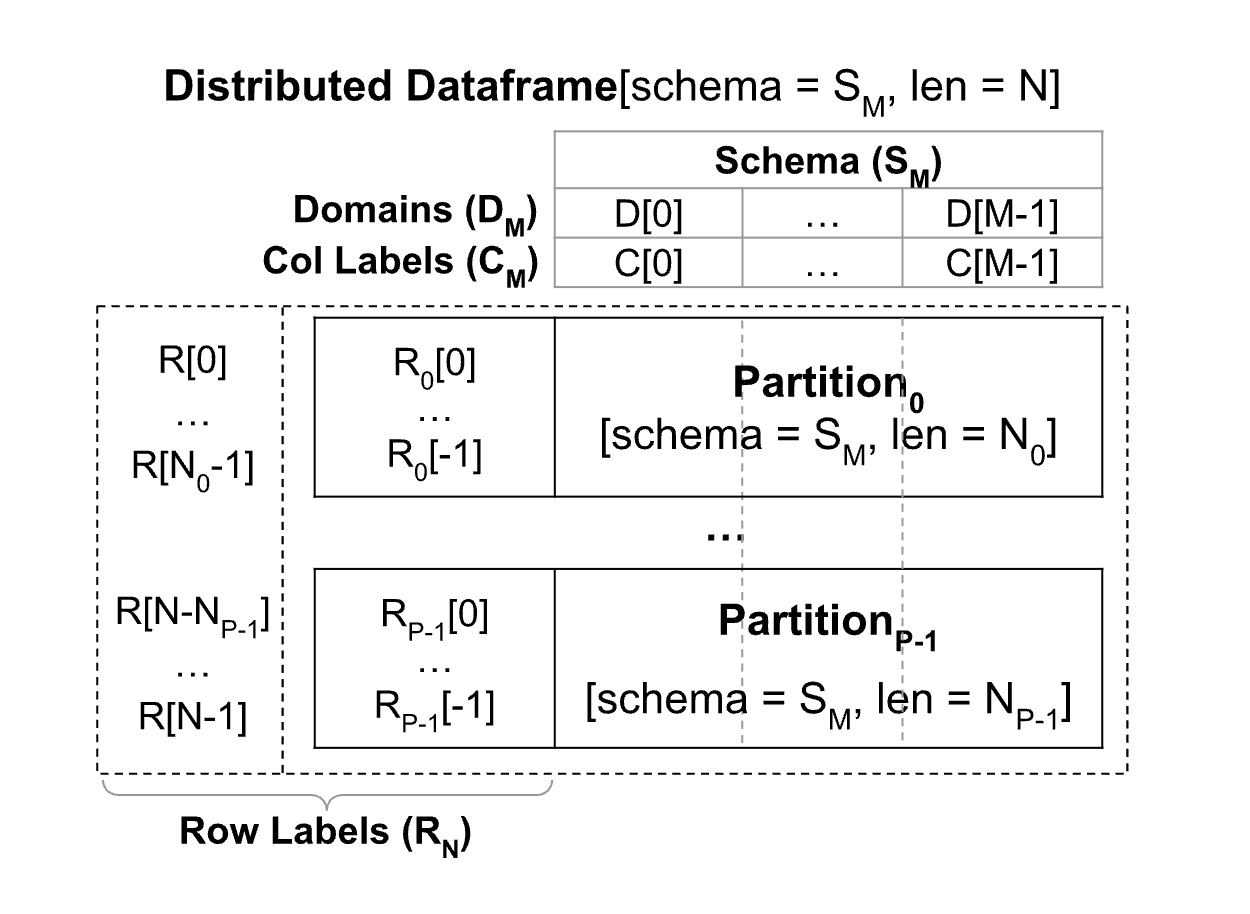
\includegraphics[width=\linewidth]{source/Figure/distDataframe.png}
    \end{center}
    \caption{Distributed Memory Dataframe (DDMF)\cite{pererathesis}}
    \label{fig:distdataframe}
\end{figure}

The Cylon channels API implements the AllToAll operation as point-to-point communication and uses the UCC library for  collective operations such as AllGather.  Distributed operators are implemented generically within Cylon.  The experiments detailed in the next section use the Distributed Join DataFrame operator.  For this case, the process follows: 1) Hash applicable columns into partitioned tables, 2) Use AllToAll to send tables to the intended destination, and 3) Execute a local join on the received tables\cite{shan2022hybrid}.

The initialization or bootstrapping of the Cylon UCX/UCC communicator necessitates the provision of communication metadata during startup. This metadata includes each process's world size, rank, and endpoint address. We utilize the \textit{Redis} key-value store to facilitate this exchange. Our design increments an atomic value to represent the rank. Before incrementing the value, the rank is set. Redis is launched externally to the Cylon processes. The only requirement is that the \textit{Redis} host be provided before initializing the Cylon runtime. Our experiments employed a combination of AWS ElastiCache, Redis, and ECS tasks that include the dockerized \textit{Redis} runtime. Depending on the specific experiment’s communication requirements, we selected a combination of \textit{Redis} deployments. One implementation limitation is that the stored metadata on \textit{Redis} must be cleared between subsequent experiments. Otherwise, the experiment executes non-deterministically and ultimately fails. In the case of executing N experiments of a given class (e.g., world size of 8 for 9.1 million rows), we need to configure N \textit{Redis} hosts when running experiments in parallel.

\begin{figure}[ht]
    \begin{center}
    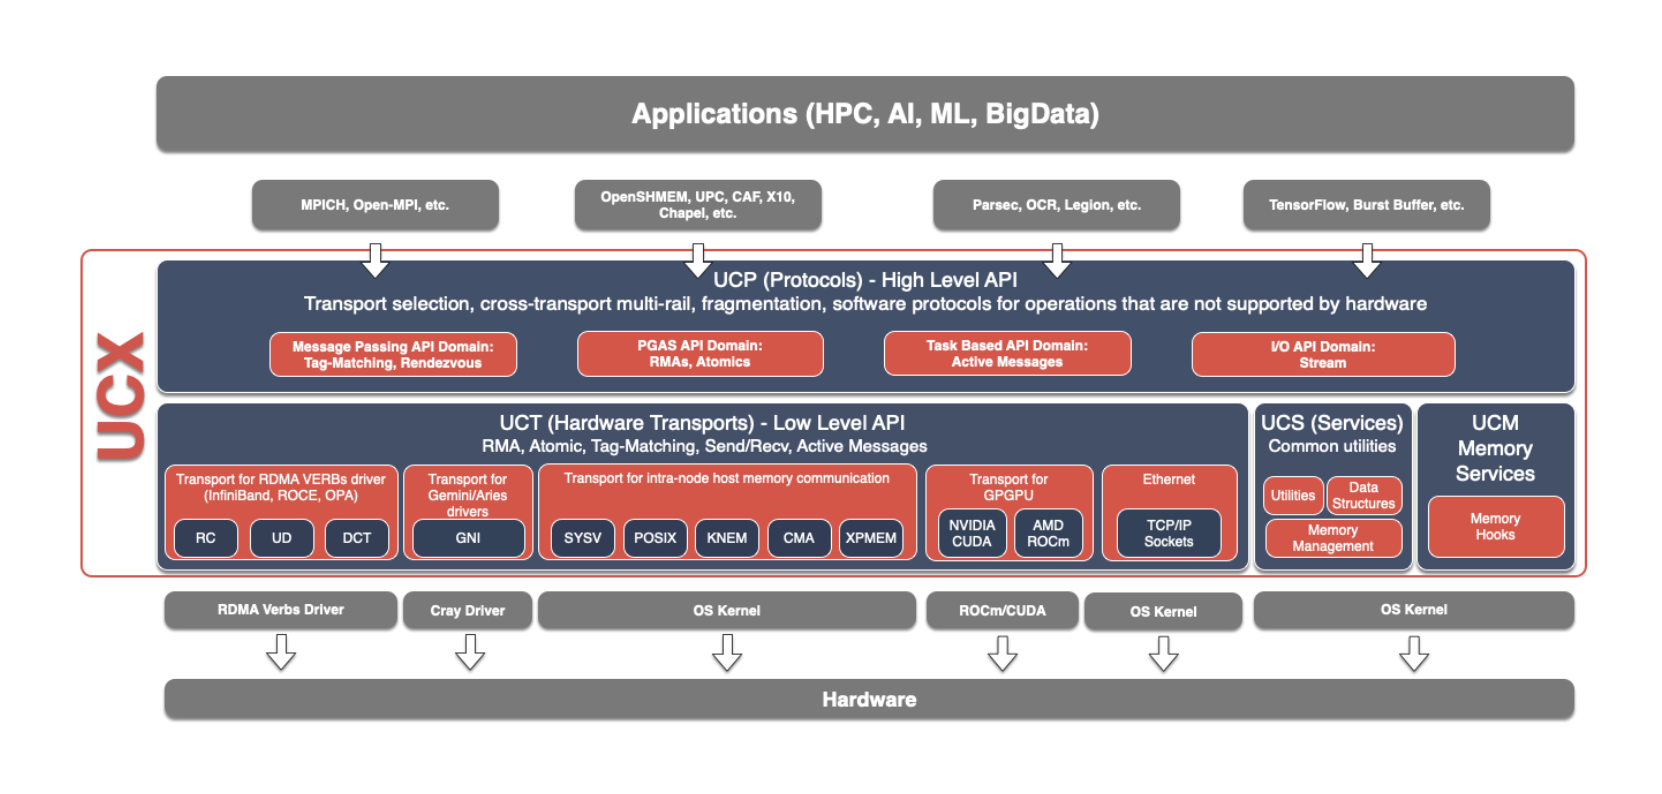
\includegraphics[width=\linewidth, height=200pt]{source/Figure/ucxarchitecture.png}
    \end{center}
    \caption{Unified Communication X (UCX) Library Architecture\cite{shamis2015ucx}}
    \label{fig:ucxarch}
\end{figure}

Our experiment design, which utilized UCX/UCC, proved highly effective for most AWS and HPC experiments. One aspect of our design involved using Docker. This product uses OS-level virtualization to deploy software in packages or containers to create a runtime environment that could be seamlessly deployed across both HPC and AWS\cite{dockerwiki}. We pushed our Dockerized environments to Dockerhub and employed Apptainer on Rivanna to construct a Singularity container encapsulating the Cylon runtime. A significant advantage of this approach is that modifications to the environment (or Dockerfile) were not required. Consequently, all our experiments utilized the same runtime, resulting in a consistent and derivative approach across infrastructure.  We believe our architecture and the inclusion of UCX/UCC to be a novel contribution, and based on our research, it is the only case we could find where UCC/UCX was being used for ML/AI pipelines such as Cylon.

A crucial aspect of this research involves executing data engineering pre-processing on serverless compute. For this subset of our study, we made a minor modification to the UCX Unified Communication Transport (UCT) lower-level API. This change was necessary due to UCX’s initialization behavior. UCX employs low-level system calls to select the most suitable and optimal communication protocol based on the available resources. However, only TCP is supported for serverless computing. We observed that the UCX device query incorrectly retrieved the incorrect IP address from the hardware during initialization. To ensure successful initialization, we had to override the IP address discovered by UCX. This modification enabled us to conduct experiments on AWS Fargate, a serverless Docker running on ECS, a fully managed container orchestration service. Unfortunately, this capability was deprecated due to changes in the underlying serverless architecture implemented by AWS.  This led us to investigate other potential communication options for BSP systems that run on serverless systems.

A similar issue was encountered with AWS Lambda functions, a serverless compute service or Function as a Service (FaaS) that allows code to execute in response to events and automatically manages and scales resources. We could not leverage the IP address override capability mentioned above to execute Cylon on AWS Lambda due to the unavailability of system calls similar to AWS Fargate. One solution presented by Copik et al. was to use NAT traversal or TCP hole punching to enable direct communication between a pair of AWS Lambda functions via the FMI library. Unlike storage-based solutions, direct communication increases communication time by multiple orders of magnitude.  Figure \ref{fig:natholepunching} illustrates this process.  NAT hole punching requires functions to be behind a NAT gateway.  The gateway hides the addresses of each function by rewriting the internal addresses with an external address.  Outgoing communication creates an entry in the translation table.  This results in replies being sent to the intended recipient.  The NAT Gateway will drop packets routed to addresses not found in the translation table.  In order to support NAT hole-punching, a publicly accessible server is required that creates entries in the translation table and relays addresses between two functions.  


\begin{figure}[ht]
    \begin{center}
    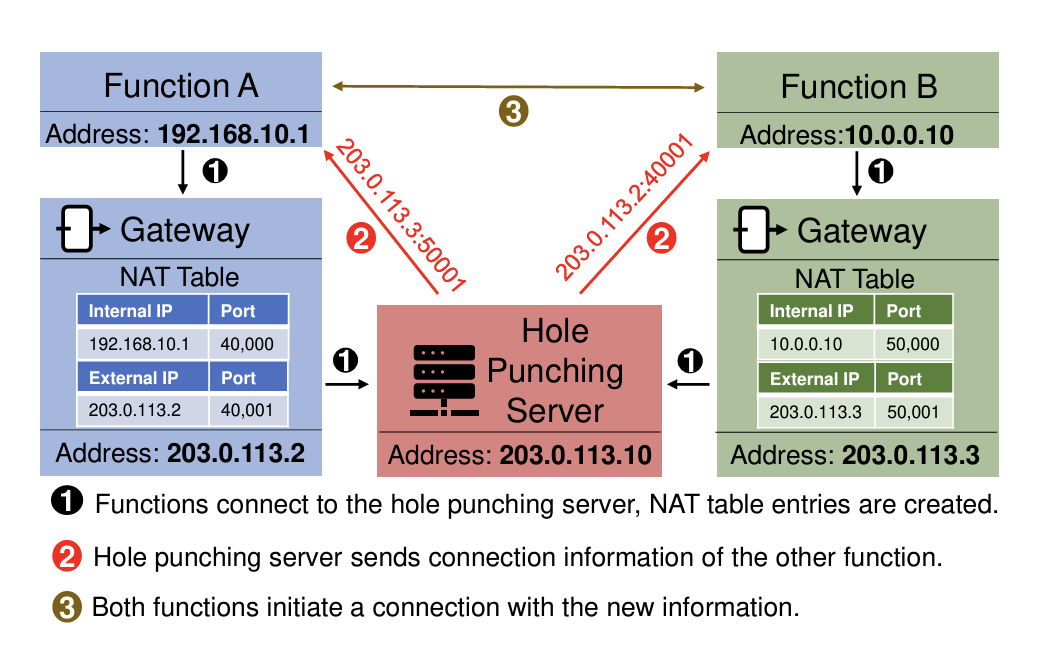
\includegraphics[width=\linewidth]{source/Figure/NatHolePunching.png}
    \end{center}
    \caption{Network Address Translation (NAT) Hole Punching\cite{copik2023fmi}}
    \label{fig:natholepunching}
\end{figure}

We created an ECS or Docker image with a C++ implementation of a relay or rendezvous server for our experiments.  Our initial goal was to integrate the FMI library into Cylon as a modification of the existing TCP UCT UCX source.  Unfortunately, this approach yielded unsuccessful results based on the UCX TCP architecture and NAT hole-punching address exchange semantics.  We believe an ideal approach is implementing FMI as a separate Cylon communicator, similar to the UCC/UCX communicator described above.  We successfully recreated and validated the FMI library's capability as a custom AWS Python Lambda Docker image.   For this work, we created a Dockerfile with all the libraries necessary for experiment execution.  We also implemented the AWS Lambda interface and created derivative experiments like the distributed join experiments detailed in the next section.  Including this library is an ideal choice based on the limitations imposed by AWS Lambda and the fact that a higher-level abstraction is necessary for direct communication between Lambda functions.  There are also cost considerations based on the AWS Lambda cost model, where request rate, execution time, and function size correlate to the overall cost.  Direct communication leads to optimized usage of Lambda functions and allows full usage of the available provisioned CPU and memory.

\begin{figure}[ht]
    \begin{center}
    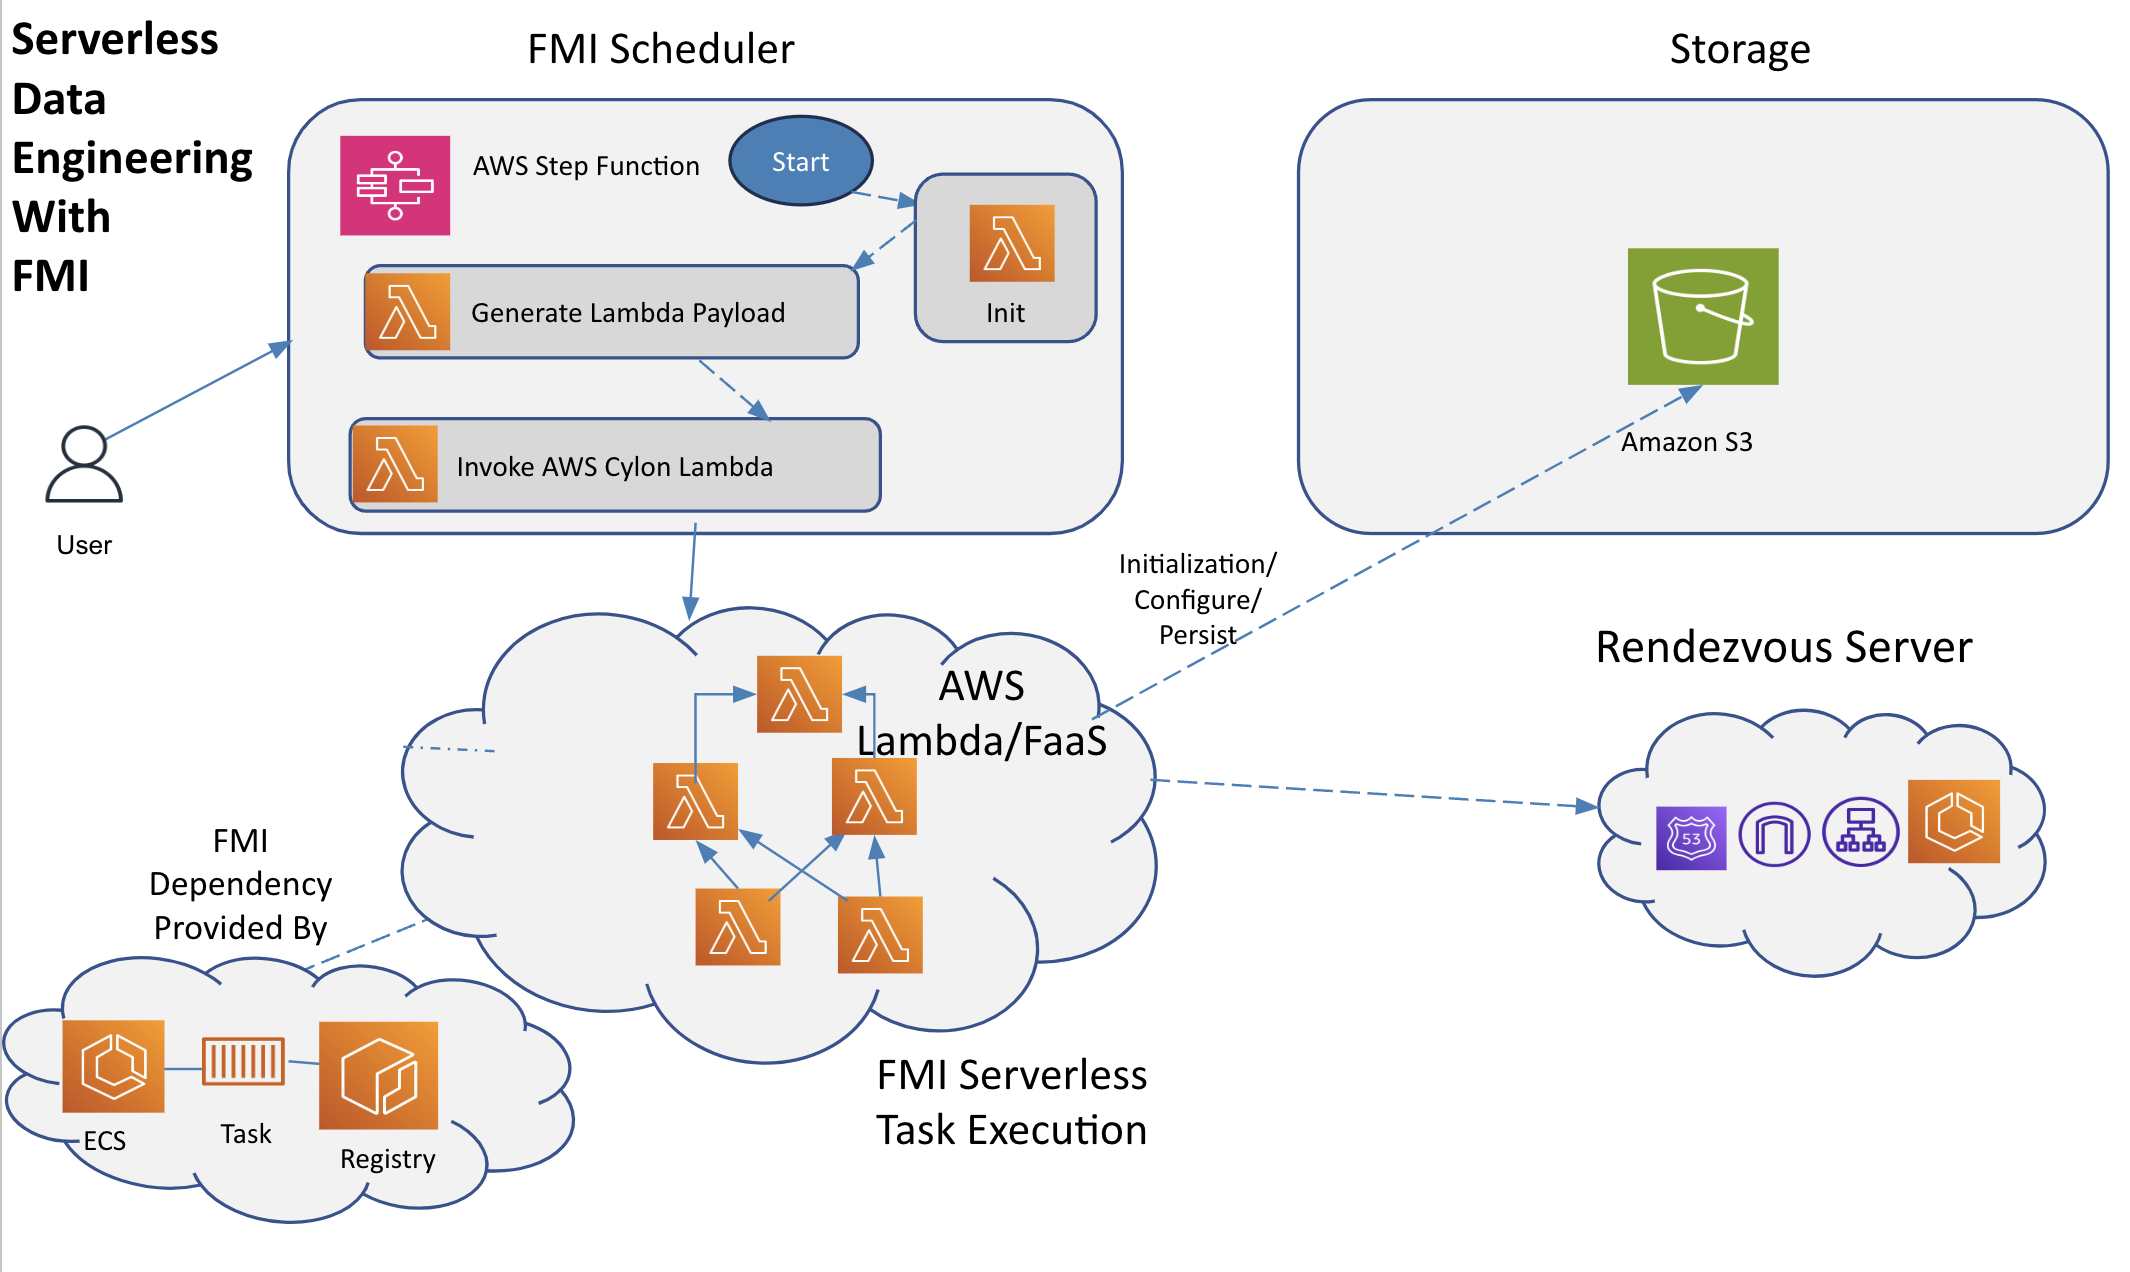
\includegraphics[width=\linewidth]{source/Figure/serverlessdataengineering.png}
    \end{center}
    \caption{Serverless Data Engineering Architecture}
    \label{fig:serverlessdataengineering}
\end{figure}

Figure \ref{fig:serverlessdataengineering} illustrates our architecture. To implement the FMI scheduler, we created an AWS Step Function, as depicted in Figure \ref{fig:fmistatemachine}. AWS Step Functions are a Software as a Service (SaaS) feature that facilitates the orchestration of AWS services into serverless workflows. The \textit{Lambda: init} start function receives a payload containing various parameters, such as the number of rows, world size, number of iterations, target S3 bucket, script, and output paths. We utilize a specific S3 bucket and push the invocation results to a folder using the \textit{Boto3} library. This approach is advantageous over parsing the data output from log files in AWS CloudWatch, a SaaS metrics repository created and utilized by AWS services, as it would be cumbersome. The Lambda init function sends the input JSON payload to the \textit{fmi\_init} AWS Lambda function. This function validates the rendezvous server’s availability and generates an N-sized array of JSON payloads, which are then sent to the \textit{Map}, \textit{ExtractAndInvokeLambda} states. The \textit{Map} state includes inline and distributed processing modes.   We choose the Distributed processing mode to enable highly parallel execution. Next, each generated payload is sent to the Lambda: Invoke state from the pass \textit{ExtractAndInvokeLambda} state.  This state passes the input to output, which executes the \textit{fmi\_executor} AWS Lambda function. The runtime of the \textit{fmi\_executor} function includes the runtime described earlier, which includes the FMI library. The incoming payload specifies the location of the target script in the S3 bucket. Upon execution of the Lambda function, the contents of the specified S3 bucket are retrieved and persisted into temporary ephemeral storage. Subsequently, Python3 executes the script used for our experiments (i.e., scaling.py). We support a single script and a folder containing Python scripts and modules. For our experiments, we combined FMI and Cylon experiments in our scaling.py Python script to facilitate execution across serverless, serverful, and HPC environments\cite{cloudmeshcommon}. 



\begin{figure}[ht]
    \begin{center}
    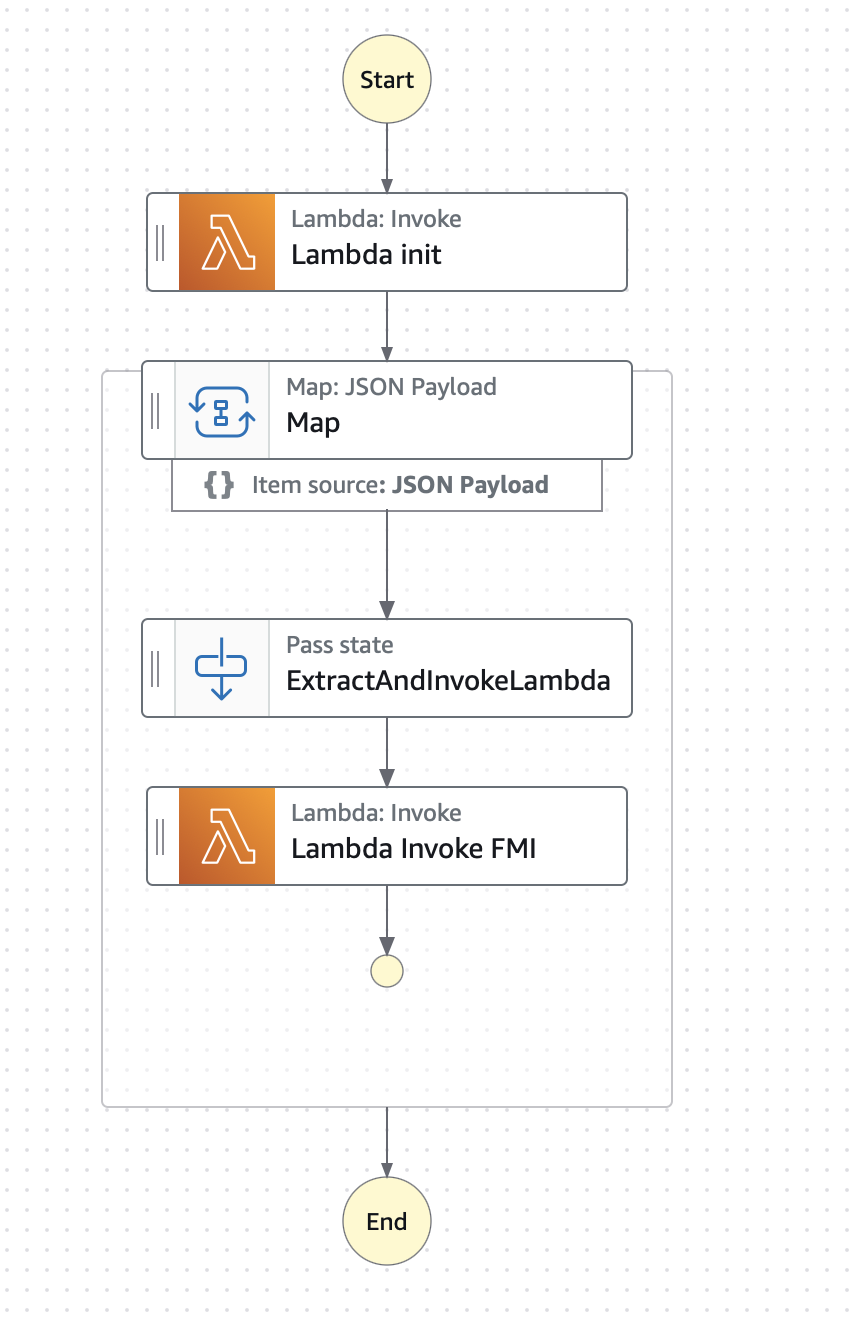
\includegraphics[width=\linewidth]{source/Figure/FMIStateMachine.png}
    \end{center}
    \caption{AWS Step Function for Serverless Data Parallel Task}
    \label{fig:fmistatemachine}
\end{figure}


During execution, the \textit{fmi\_executor} connects with the Rendezvous Server referenced in Figure \ref{fig:serverlessdataengineering}.  Once the second function in the pair connects to the Rendezvous Server, both servers receive the destination function's public address.  The Python script then continues to execute until the collective operation is performed.  For the experiments discussed below, we use an AllReduce collective to calculate a summation of start-to-end execution across the world size of executing functions.  We also use the cloudmesh stopwatch library to facilitate logging and benchmarking the runtime of our executing experiments.